\documentclass[12pt, a4paper]{extarticle}


% Russian text support
\usepackage[T2A]{fontenc}
\usepackage[utf8]{inputenc}
\usepackage[russian]{babel}

% Some useful packages
\usepackage{indentfirst}
\usepackage{etoolbox}
\usepackage{amsmath}
\usepackage{amssymb}
\usepackage{amsfonts}
\usepackage{tabularx}

% Pictures support
\usepackage{graphicx}
\graphicspath{ {./images/} }

% Page geometry
\usepackage[
    left=3cm,
    right=1cm,
    top=2cm,
    bottom=2cm
]{geometry}

% Code
\usepackage{listings}
\usepackage{xcolor}

\definecolor{codegreen}{rgb}{0,0.6,0}
\definecolor{codegray}{rgb}{0.5,0.5,0.5}
\definecolor{codepurple}{rgb}{0.58,0,0.82}
\definecolor{backcolour}{rgb}{1,1,1}

\lstdefinestyle{codestyle}{
    backgroundcolor=\color{backcolour},   
    commentstyle=\color{codegreen},
    keywordstyle=\color{magenta},
    numberstyle=\tiny\color{codegray},
    stringstyle=\color{codepurple},
    basicstyle=\ttfamily\footnotesize,
    breakatwhitespace=false,         
    breaklines=true,                 
    captionpos=b,                    
    keepspaces=true,                 
    numbers=left,                    
    numbersep=5pt,                  
    showspaces=false,                
    showstringspaces=false,
    showtabs=false,                  
    tabsize=2,
    extendedchars=\true,
}

\lstset{style=codestyle}

% Make titles not to have numbering
\newenvironment*{dummyenv}{}{}

\newcommand{\mysection}[1]{
    \addcontentsline{toc}{section}{#1}
    \begin{dummyenv}
        \bfseries\large #1
    \end{dummyenv}
}

\makeatletter
\patchcmd{\l@section}
  {\hfil}
  {\leaders\hbox{\normalfont$\m@th\mkern \@dotsep mu\hbox{.}\mkern \@dotsep mu$}\hfill}
  {}{}
\makeatother

% Some useful stuff
\newcommand{\Answer}[1]{\textbf{Ответ:} #1}

\newcolumntype{Y}{>{\centering\arraybackslash}X}

% Here we go...
\title{БДЗ по прикладной криптографии}
\author{Фирсов Георгий, М21-507}

\begin{document}

\maketitle

\tableofcontents

\pagebreak
\mysection{Задание 1}

При известном заранее значении $D$ нарушитель может единожды найти такое значение $z$, что:
\begin{equation}
    \texttt{SHA256}(z) < \frac{2 ^ n}{D}.
\end{equation}

Это потребует некоторого времени, но идея в том, что это делается единожды и заранее.

Далее при обнародовании $x$ нарушитель вычисляет $y = z \oplus x$. При этом верна следующая
цепочка:
\begin{equation}
    H(x, y) = H(x, x \oplus z) = \texttt{SHA256}(x \oplus x \oplus z) = 
        \texttt{SHA256}(z) < \frac{2 ^ n}{D},
\end{equation}
то есть нарушитель может для каждого $x$ найти такой $y$, что $H(x, y) < \frac{2 ^ n}{D}$
за некоторое константное время.
\\

\mysection{Задание 2}

\begin{enumerate}
    \item На рисунке \ref{fig:2.1} представлен процесс вычисления хэша $R_i$ (или просто искомого
        коммитмента $S$), входящего в заголовок $i$-го блока, при помощи троичного дерева Меркла. 
        Фактически это достаточно очевидное само по себе переложение процесса вычисления на 
        троичное дерево вместо двоичного.
        \begin{figure}[h!]
            \centering
            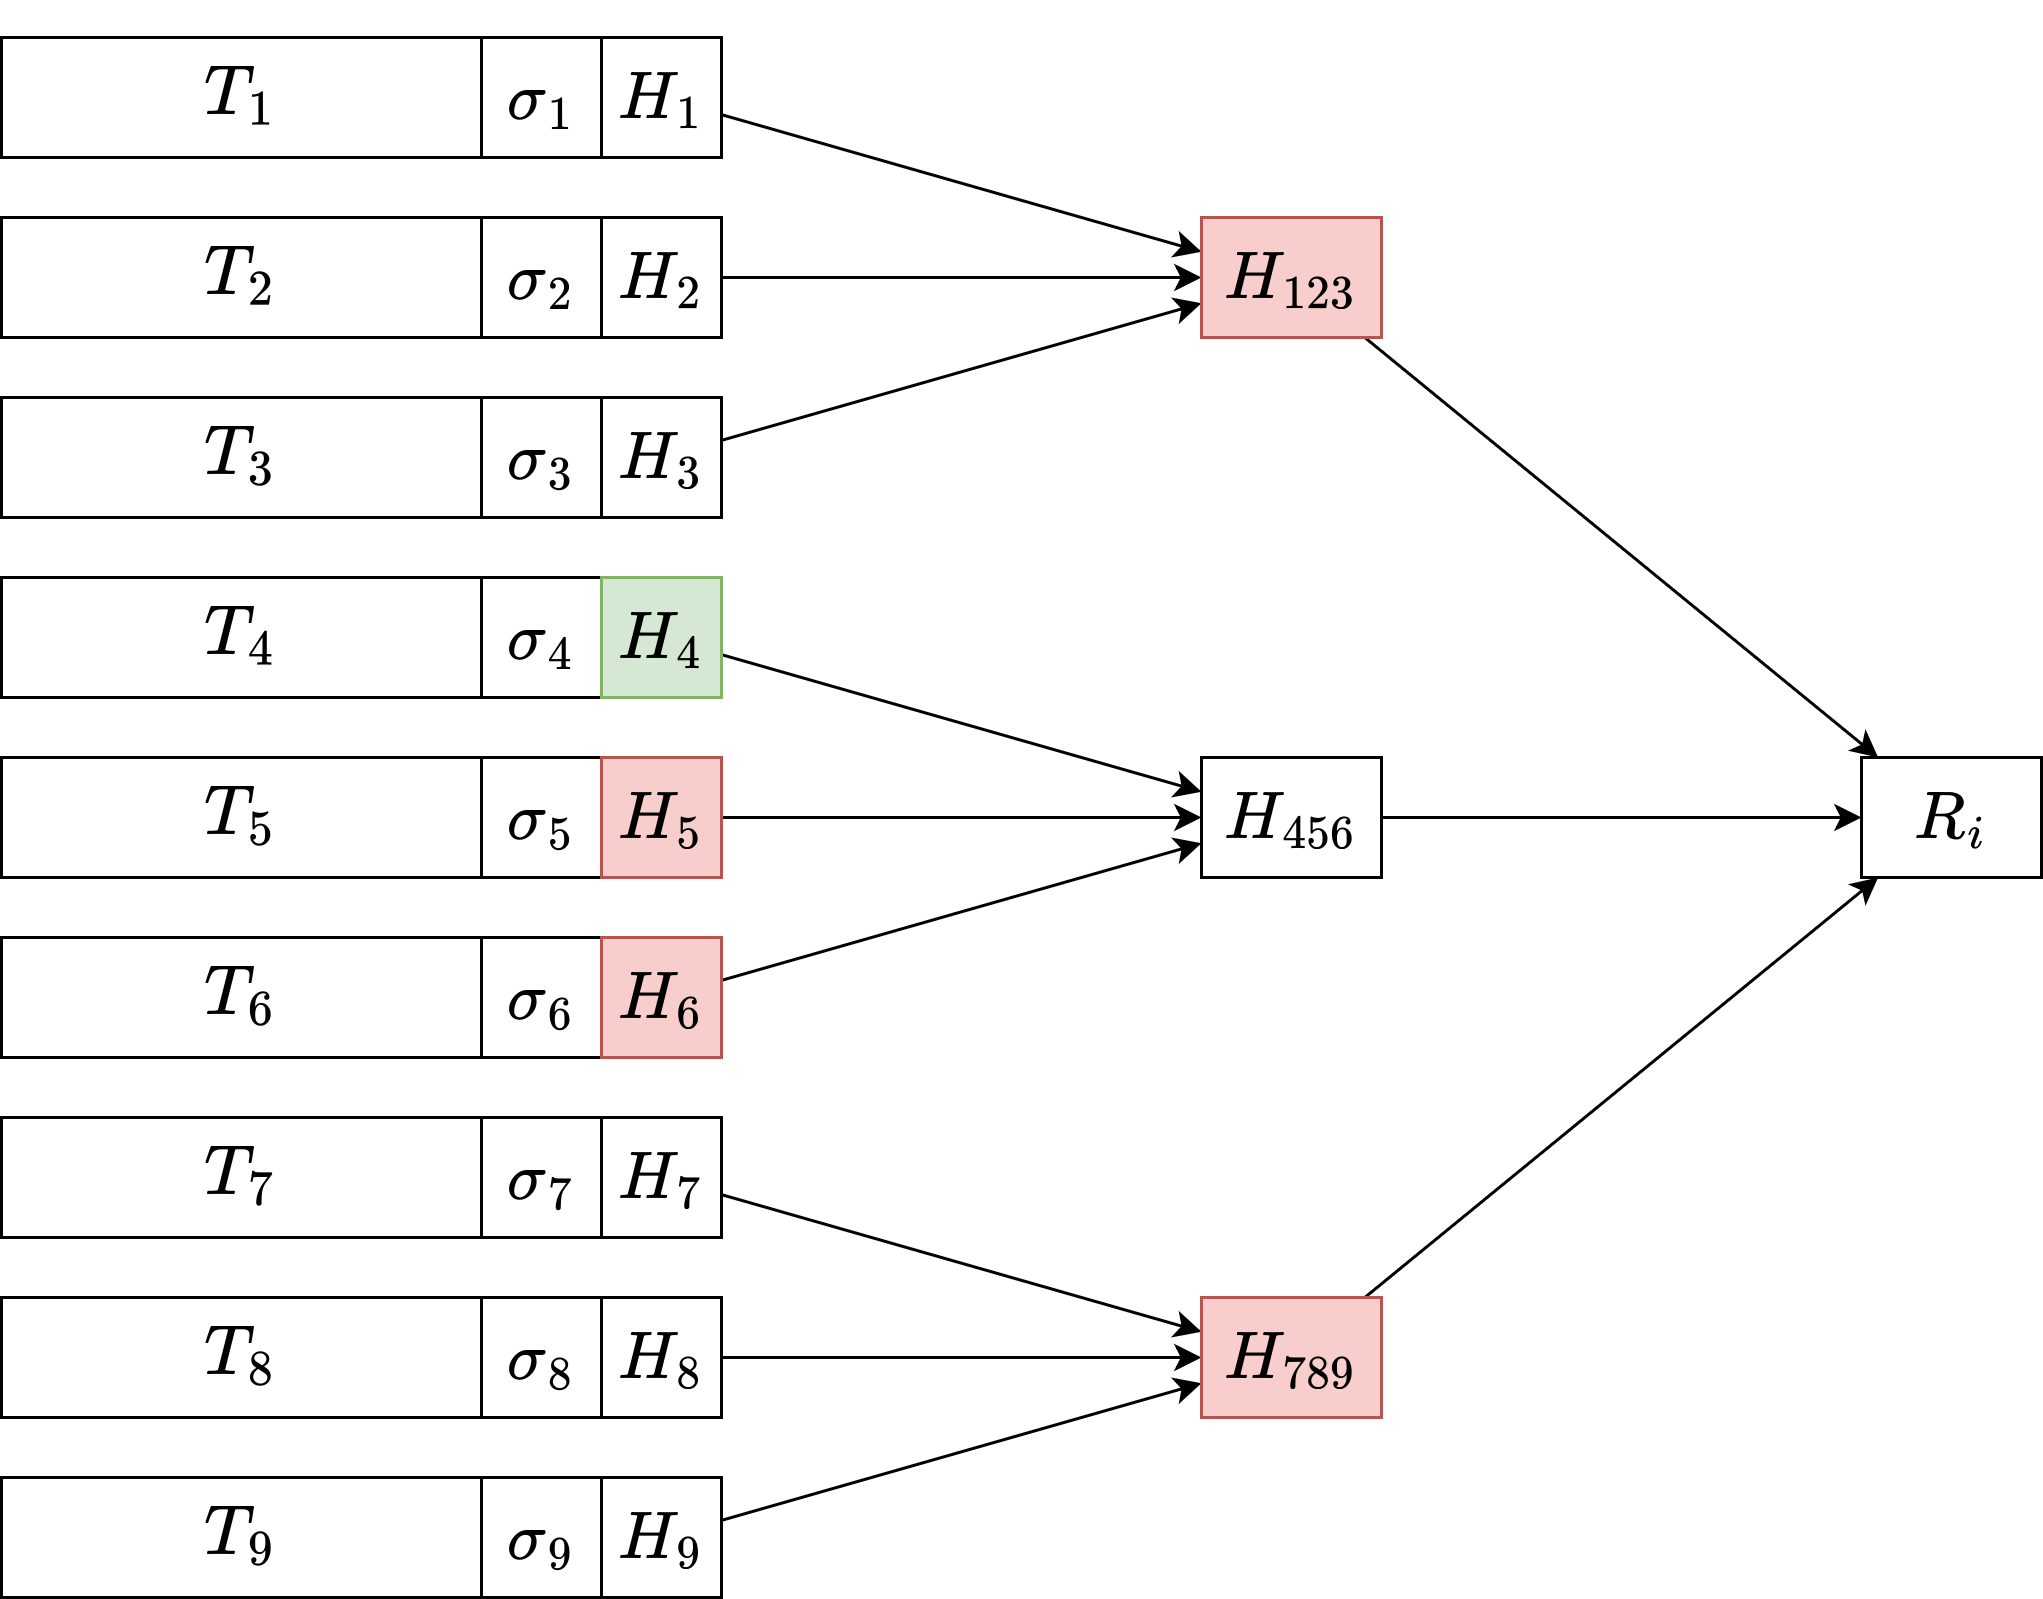
\includegraphics[width=\textwidth]{2.1.png}
            \caption{Схема вычисления хэша при помощи троичного дерева Меркла}
            \label{fig:2.1}
        \end{figure}
        
        Для того, чтобы доказать вхождение транзакции $T_4$ (хэш которой выделен зеленым на рисунке
        \ref{fig:2.1}) требуется предоставить Борису следующие значения: $H_5$, $H_6$ (соседние
        хэши) и $H_{123}$, $H_{789}$ (хэши соседних поддеревьев). Данные значения на рисунке
        \ref{fig:2.1} выделены красным.
        
        Борис вычисляет $\tilde{H}_{456}$ на основе известного $H_4$ и предоставленных $H_5$, $H_6$
        ($\tilde{H}_{456} = H(H_4 || H_5 || H_6)$), после чего на основе полученного значения и
        предоставленных $H_{123}$, $H_{789}$ рассчитывает $\tilde{S} = H(H_{123} || \tilde{H}_{456}
        || H_{789})$. Если $\tilde{S} = R_i$, то $T_4$ содержится в блоке (при условии, что все 
        предоставленные хэши верны, что было бы логично при доказательстве).
    \item Отметим, что путь от корня до проверяемой вершины содержит $\lceil \log_k n \rceil$
        элементов дерева. Для каждого элемента необходимо предоставить $k - 1$ хэш --- это
        хэши соседних поддеревьев (а для листового уровня --- соседние хэши-листы). Таким
        образом получается следующая формула для длины доказательства: 
        \begin{equation}
            (k - 1) \cdot \lceil \log_k n \rceil.
        \end{equation}
        
        \Answer{$(k - 1) \cdot \lceil \log_k n \rceil$}.
    \item Ясно, что для $x > 1$ выполнено: $\log_2 x < 2 \cdot \log_3 x$. Более наглядно это
        представлено на рисунке \ref{fig:2.3}:
        \begin{figure}[h!]
            \centering
            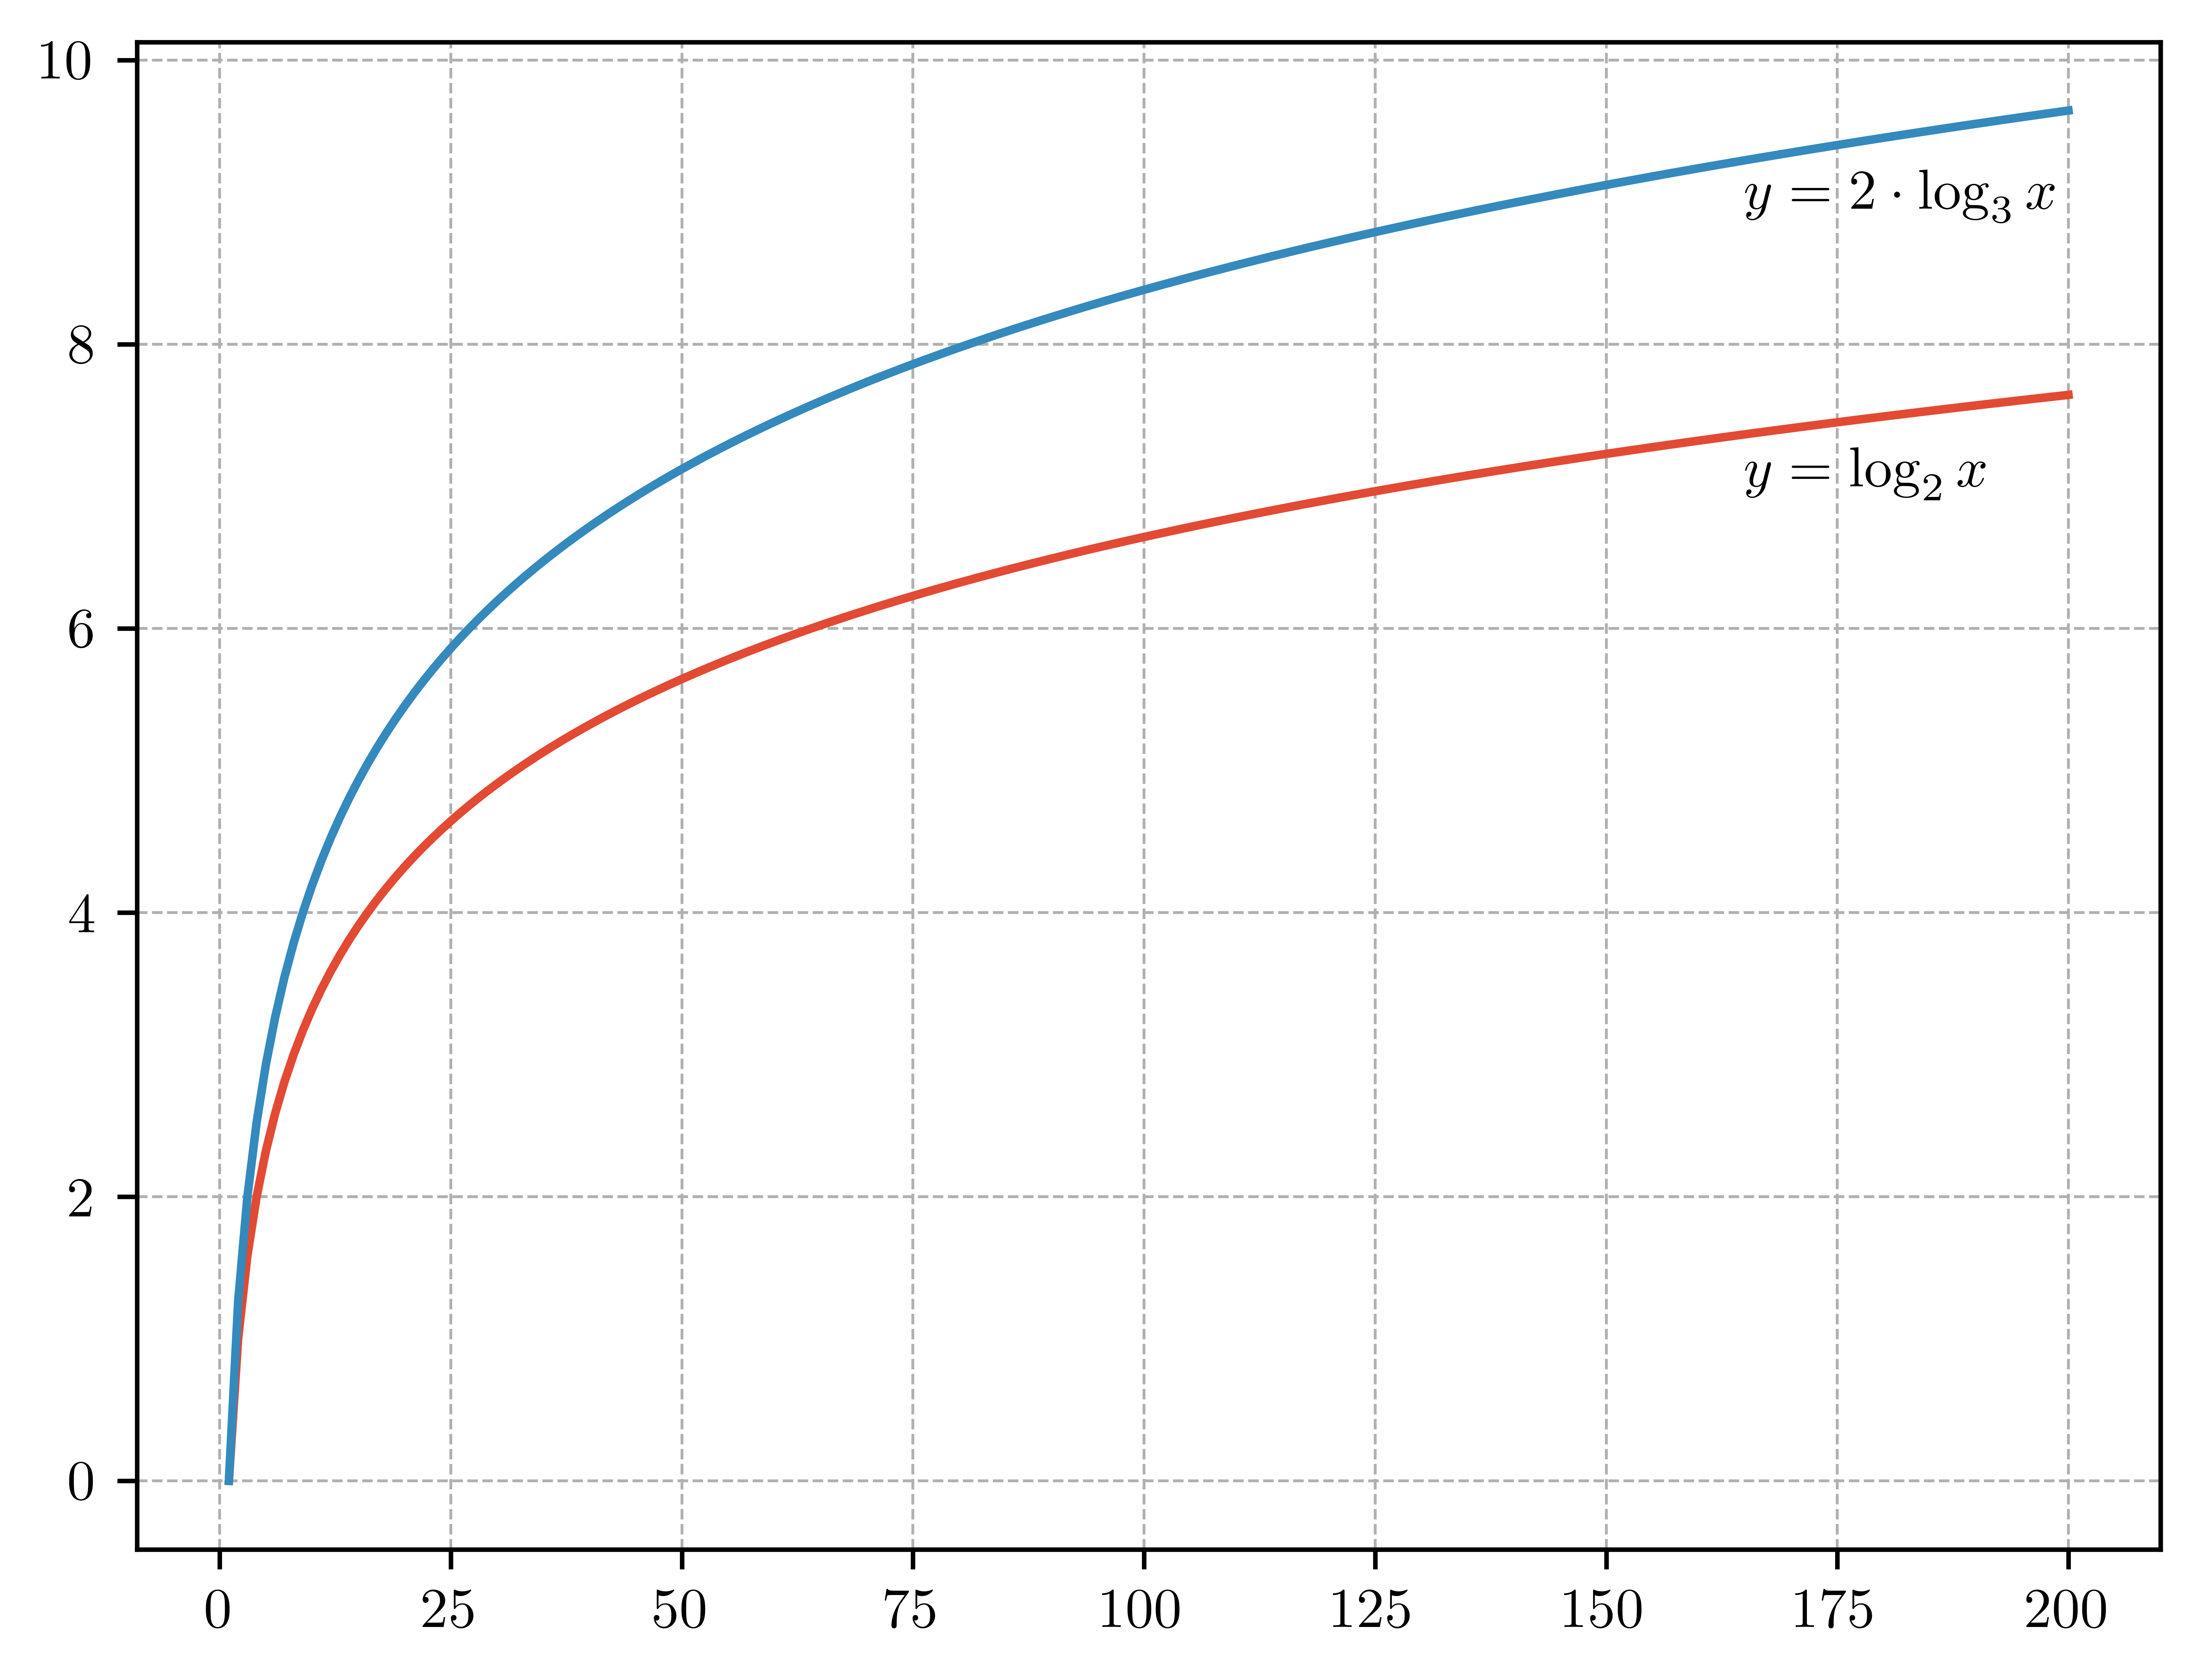
\includegraphics[width=0.7\textwidth]{2.3.png}
            \caption{графики двоичного (красная линия) и удвоенного троичного (синяя линия) 
                логарифмов в одинаковом масштабе}
            \label{fig:2.3}
        \end{figure}
        
        Из этого следует, что использование двоичного дерева Меркла эффективнее, чем троичного (и на 
        самом деле какого-бы то ни было еще), так как длина доказательства для него будет меньше.
        
        \Answer{двоичное дерево использовать оптимальнее, чем троичное}.
\end{enumerate}

\mysection{Задание 3}

Все пункты данной задачи будут для наглядности проиллюстрированы конкретным примером, на основе
которого далее будет дано обобщенное решение.

\begin{enumerate}
    \item На рисунке \ref{fig:3.1} изображена цепочка блоков: зеленым выделен блок, заголовок которого
        хранится в памяти компьютера Бориса, желтым --- блок, в который входит транзакция, для которой
        требуется доказать вхождение в цепь. Через $R_i$ обозначается хэш-вершина дерева Меркла для 
        транзакций $i$-го блока, через $H_{i - 1}$ --- хэш заголовка предыдущего (то есть с индексом 
        $i - 1$) блока.
        \begin{figure}[h!]
            \centering
            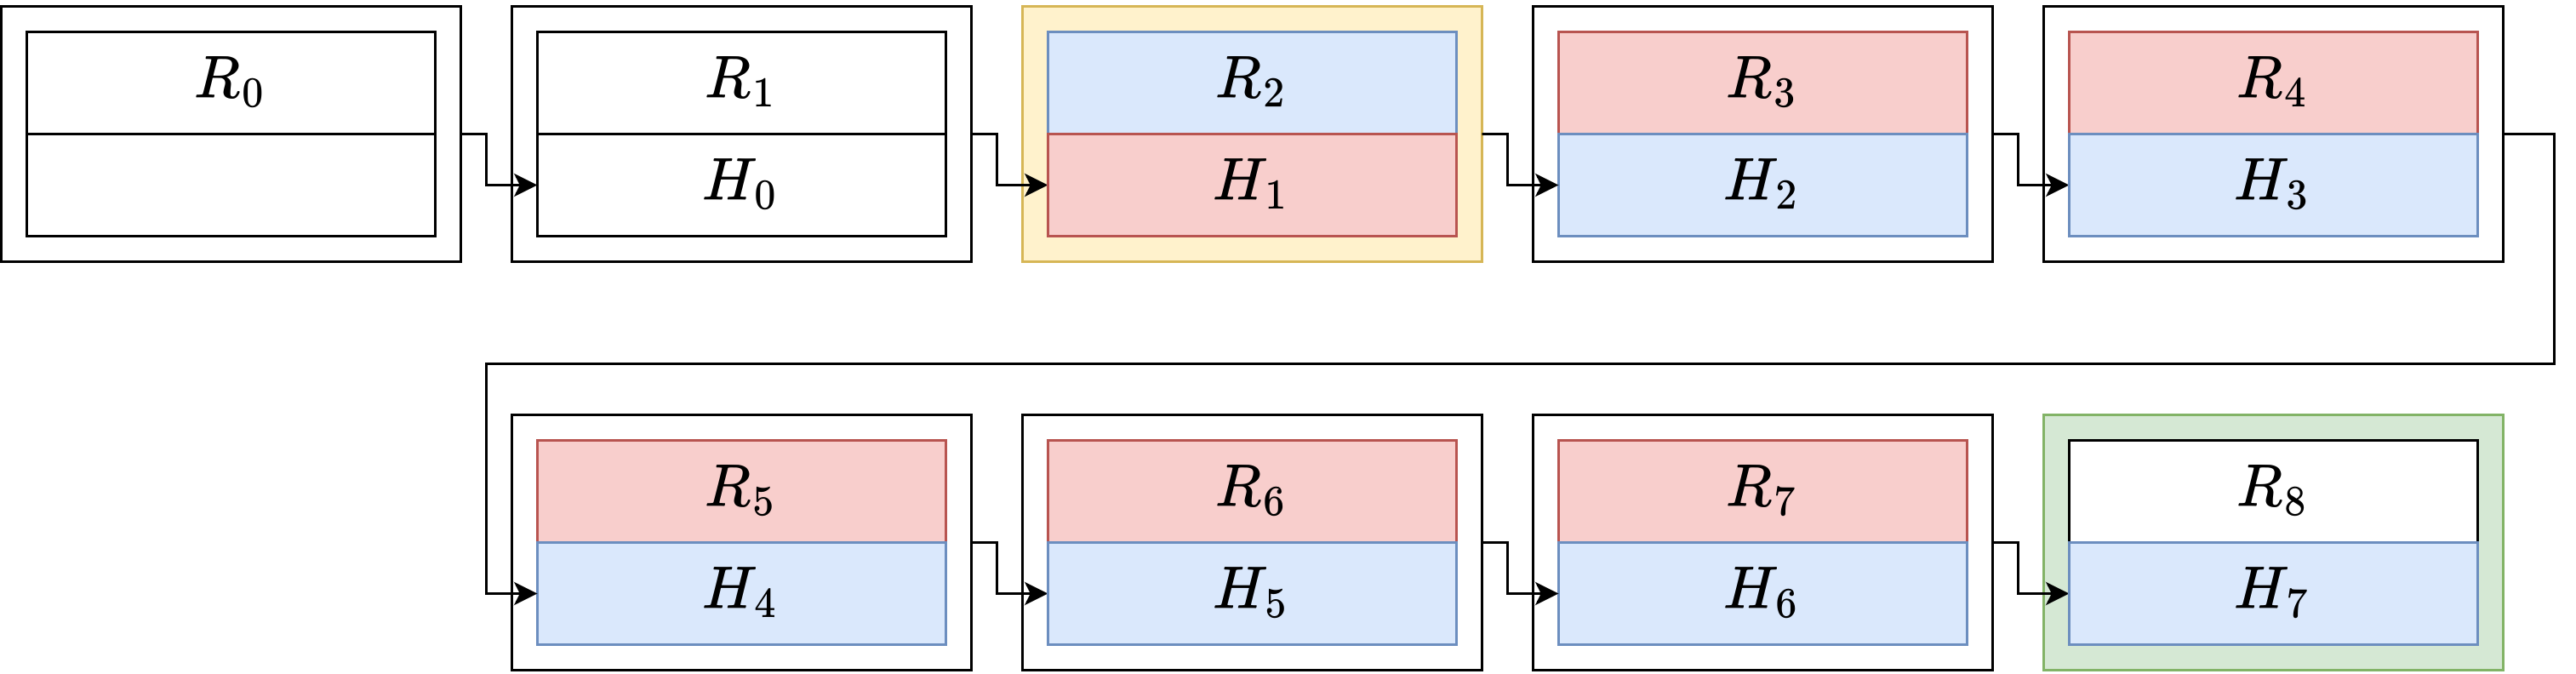
\includegraphics[width=\textwidth]{3.1.png}
            \caption{Доказательство нахождения транзакции из блока с индексом 2 в цепи}
            \label{fig:3.1}
        \end{figure}
        
        Красным цветом на рисунке \ref{fig:3.1} обозначаются данные, которые предоставляются Анной
        для доказательства, синим --- вычисляемые Борисом значения. Следует отметить, что для вычисления
        значения $R_2$ (в изображенном примере) Борису требуется получить от Анны еще 
        $\lceil \log_2 n \rceil$ хэшей для дерева Меркла (см. задачу 2). Проведем обобщение.
        
        \Answer{Анне требуется предоставить Борису следующие данные:
            \begin{itemize}
                \item $\lceil \log_2 n \rceil$ хэшей для дерева Меркла для вычисления хэша $R_i$,
                    где $i$ --- индекс блока, в который входит исследуемая транзакция;
                \item хэш заголовка предыдущего блока $H_{i - 1}$, на основе которого в совокупности с 
                    рассчитанным $R_i$ вычисляется $H_i$;
                \item хэши-вершины деревьев Меркла для блоков от $i + 1$ до $c - 1$, где $c$ --- индекс
                    <<текущего>> блока.
            \end{itemize}
        }
        
    \item Для иллюстрации данного пункта будет использоваться рисунок \ref{fig:3.1}. В этом случае $k = 6$
        (то есть прямо как и в условии). Размер хэша $32$ байта (это 256 бит SHA256). Как было сказано
        в предыдущем пункте, требуется передать:
        \begin{itemize}
            \item $\lceil \log_2 n \rceil$ хэшей для дерева Меркла: $\lceil \log_2 1024 \rceil \cdot 
                32 = 320$ байт;
            \item хэш заголовка предыдущего блока: $32$ байта;
            \item $k - 1$ хэшей-вершин деревьев Меркла блоков между блоком с транзакцией и головным:
                $(6 - 1) \cdot 32 = 160$ байт.
        \end{itemize}
        
        \Answer{$320 + 32 + 160 = 512$ байт.}
    
    \item Оптимизация происходит за счет того, что при доказательстве можно пропустить проверку
        некоторых промежуточных блоков. Пример ускорения показан на рисунке \ref{fig:3.3} для двух
        случаев: когда текущий блок у Бориса имеет индекс 8 и 9. Красной линией показан <<обходной>>
        путь, позволяющий не проверять промежуточные блоки. Так, в первом случае достаточно предоставить
        только хэши для проверки дерева Меркла генезис-блока, на основе вычисленного значения вершины
        которого вычисляется хэш заголовка $H_0$. Во втором случае текущий блок чуть дальше, а поэтому
        требуется дополнительно предоставить хэш $H_7$ и хэш-вершину дерева Меркла для предыдущего 
        блока $R_8$. При этом данные случаи являются в некотором смысле одними из самых оптимальных.
        \begin{figure}[h!]
            \centering
            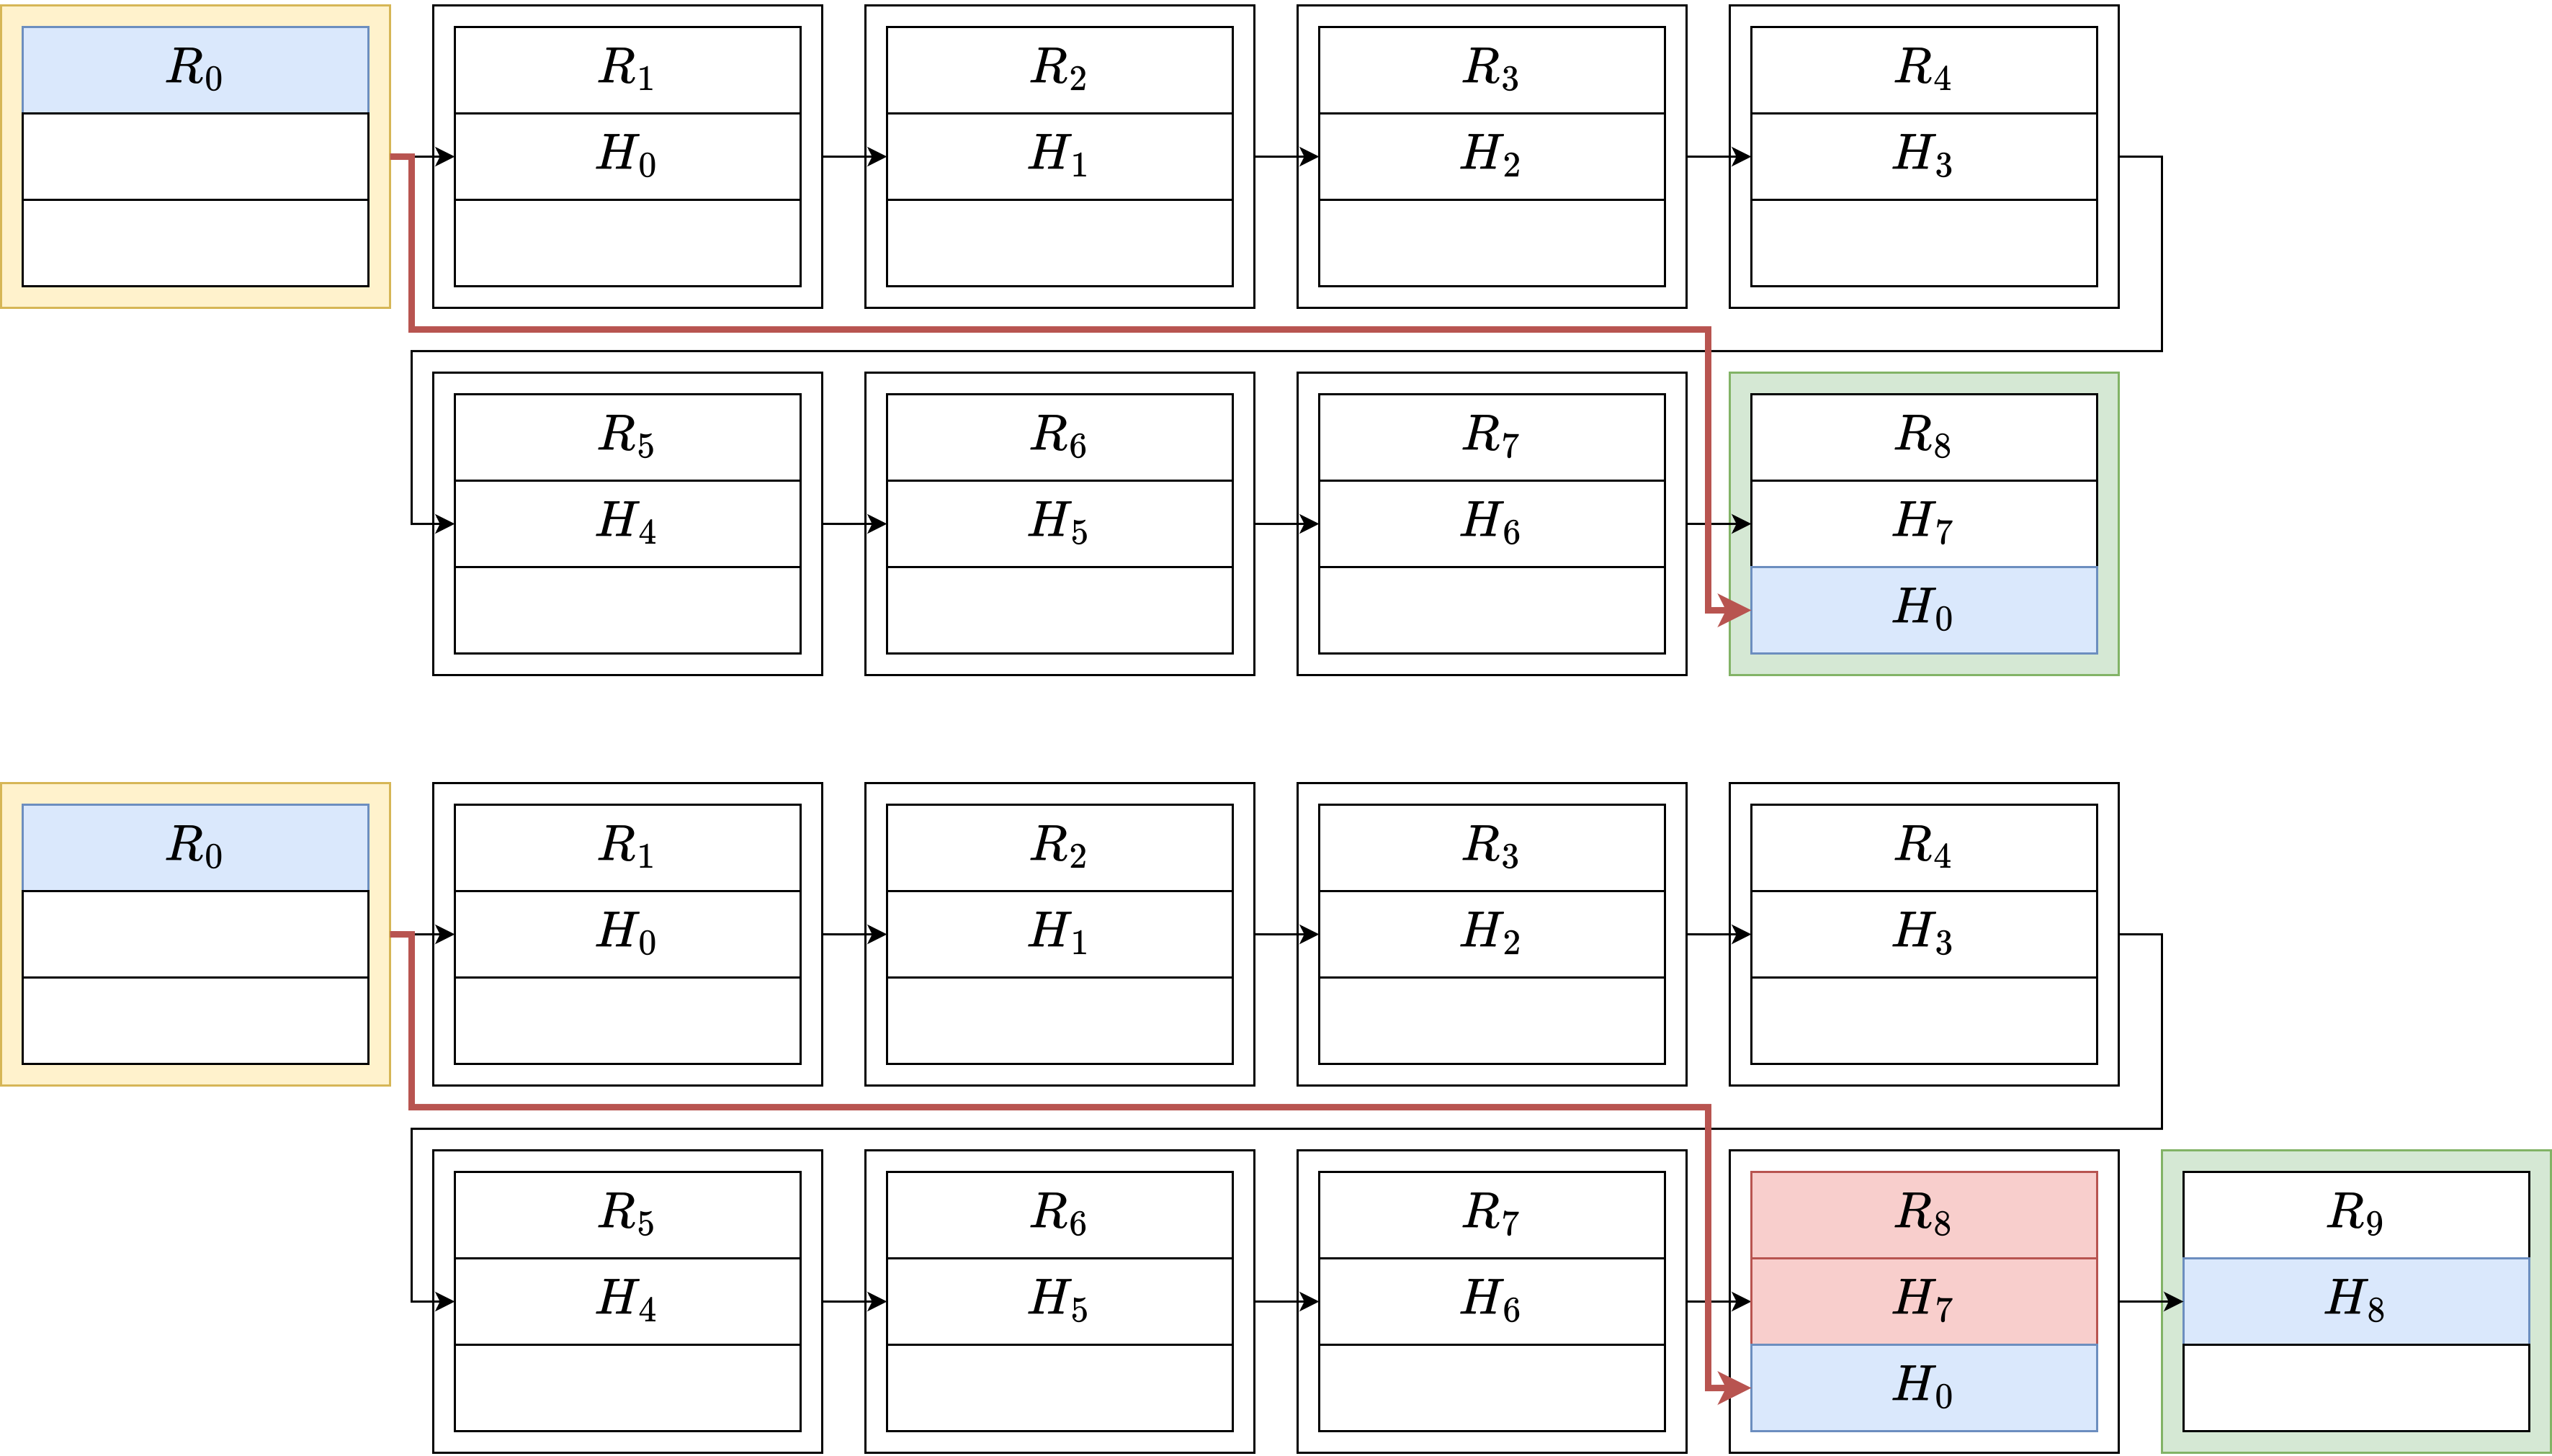
\includegraphics[width=\textwidth]{3.3.png}
            \caption{Пример оптимизации доказательства при помощи рассматриваемой схемы}
            \label{fig:3.3}
        \end{figure}
        
        Рассмотрим теперь худший случай: доказательство вхождения транзакции из блока с индексом 1
        при индексе текущего $k = 2 ^ d - 1$ для $d \in \mathbb{N}$. Рассмотрим пример <<пути>>
        проведения доказательства на более высоком уровне абстракции (рис. \ref{fig:3.3-2}). Красным
        цветом обозначены <<обходные>> пути.
        \begin{figure}[h!]
            \centering
            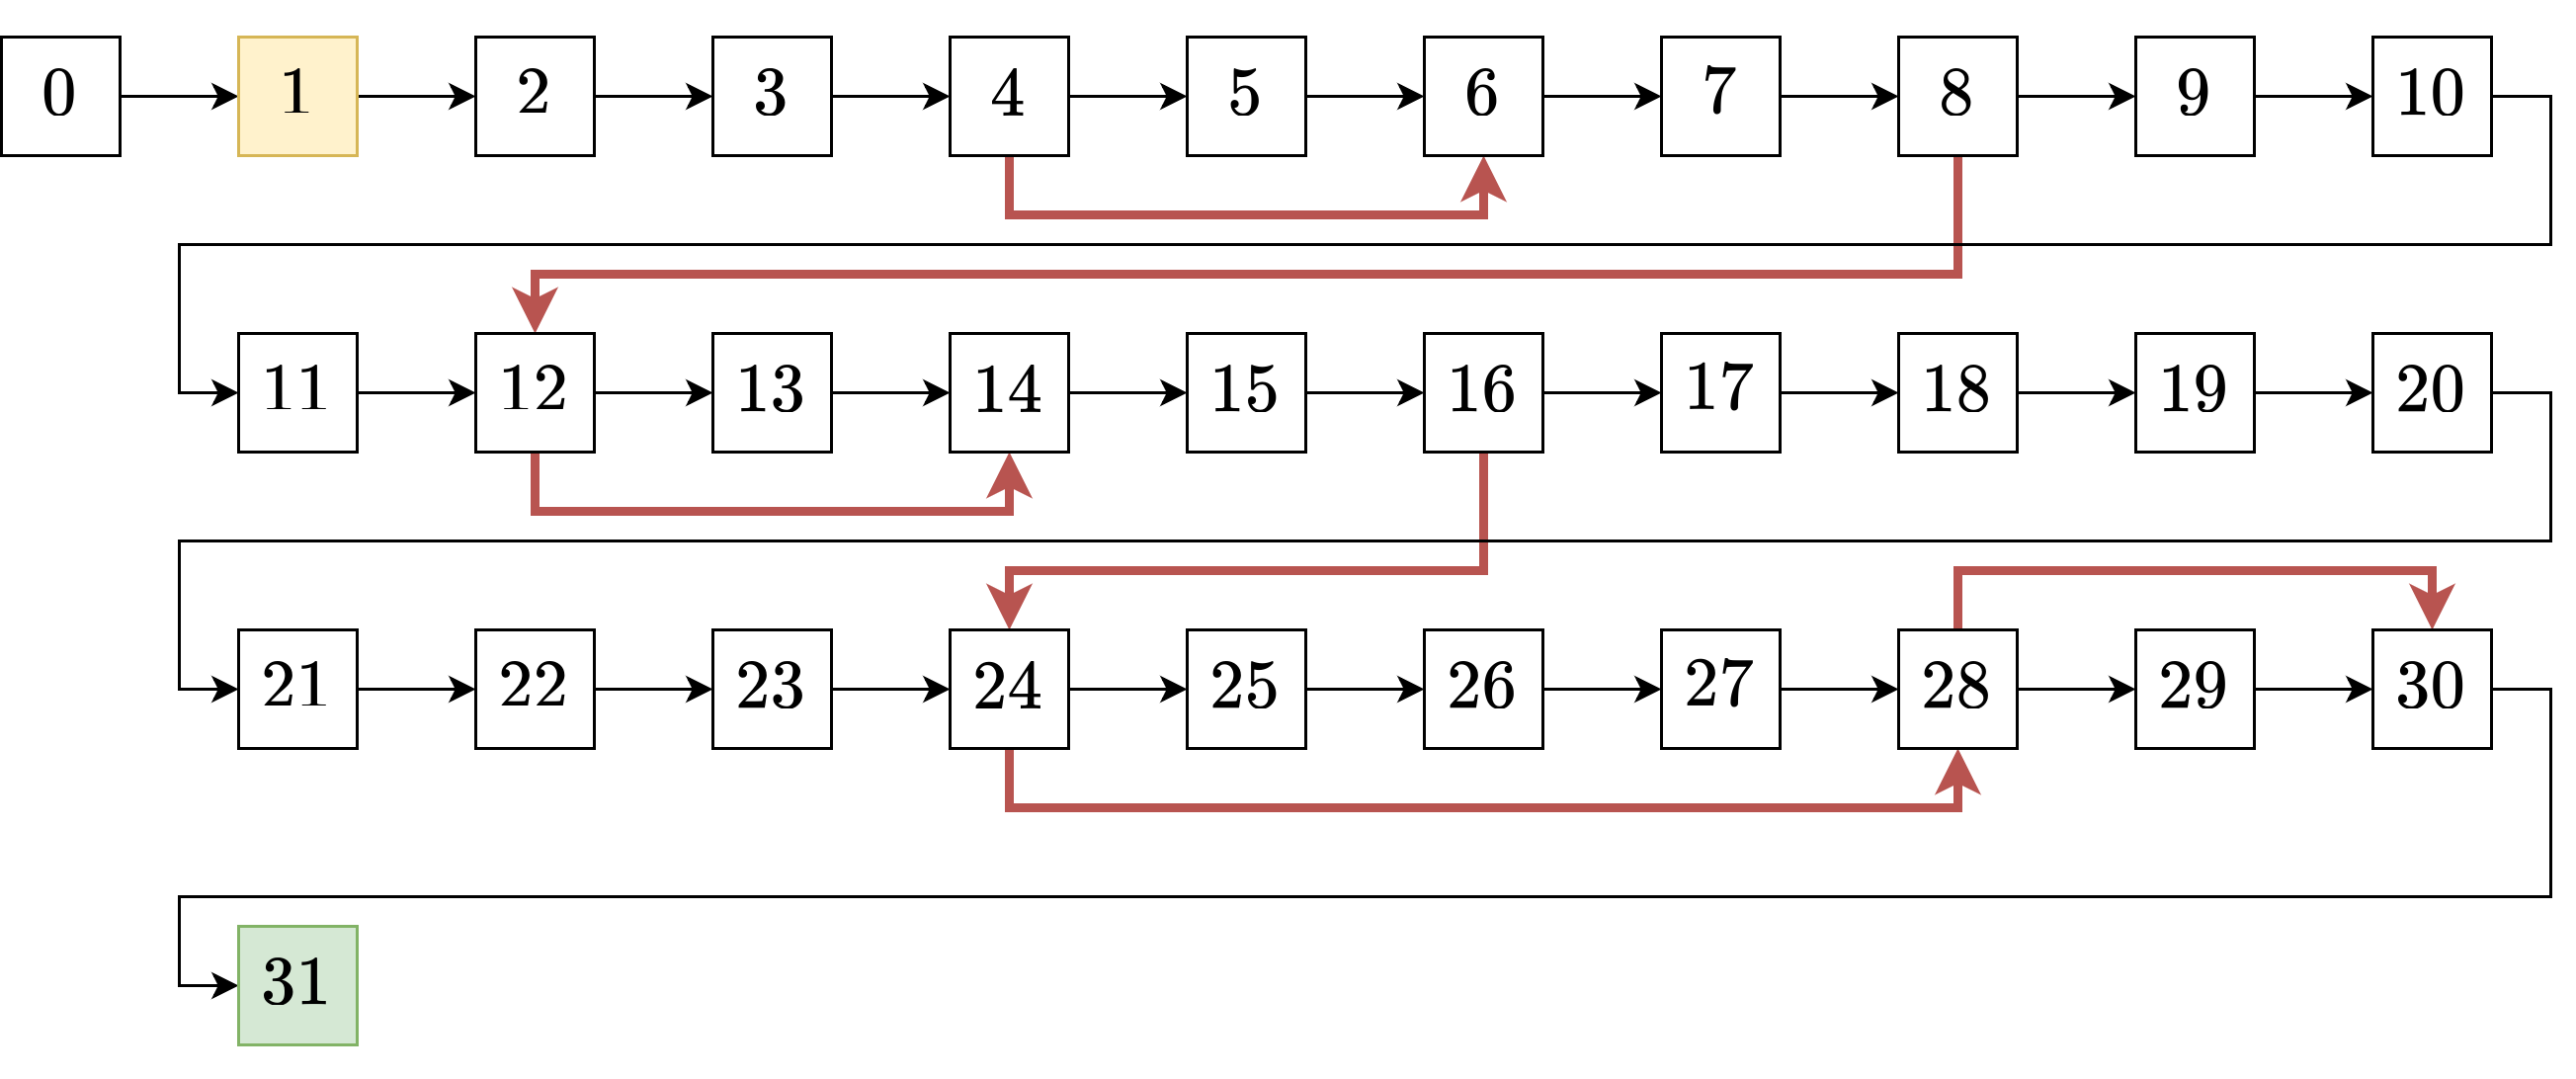
\includegraphics[width=\textwidth]{3.3-2.png}
            \caption{Пример <<худшего>> случая доказательства при помощи рассматриваемой схемы для $k = 31$}
            \label{fig:3.3-2}
        \end{figure}
        
        Как видно из рисунков \ref{fig:3.1} и \ref{fig:3.3}, один <<обычный>> переход <<стоит>> 1 хэш (только
        хэш-вершина дерева Меркла для блока, в который осуществляется переход), а <<обходной>> путь --- 2 хэша
        (тот же хэш-вершина дерева Меркла, а также хэш заголовка блока, который предшествует тому, в который
        осуществляется переход). Таким образом, полный объем доказательства составляет:
        \begin{equation}
            \mathfrak{v}(n, k) = \lceil \log_2 n \rceil + 2 \cdot \mathfrak{l}(k) + \mathfrak{s}(k),
        \end{equation}
        где $\mathfrak{l}(k)$ --- количество <<обходных>> переходов, $\mathfrak{s}(k)$ --- количество
        <<обычных>> переходов. При этом хэш заголовка генезис-блока уже учтен в данной формуле, так как
        переход от 1-го блока ко 2-му как раз ему и соответствует (в остальных случаях переход соответствует,
        как и было сказано, хэшу-вершине дерева Меркла).
        
        В приложении А предоставлен код, который для входного параметра $k$ возвращает количество 
        <<обходных>> путей, количество <<обычных>> путей (то есть путей в следующий блок) и список блоков, 
        для которых требуется доказательство правильности хэша.
        
        В таблице \ref{tbl:3.3} представлены результаты работы функции \texttt{get\_path} из приложенного
        листинга для $d = \overline{2, 15}$.
        \begin{table}[h!]
            \caption{Значения $\mathfrak{l}(k)$ и $\mathfrak{s}(k)$ для значений $k = 2 ^ d - 1$
                для последовательных значений $d = \overline{2, 15}$}
            \label{tbl:3.3}
            \begin{tabularx}{\textwidth}{|Y|Y|Y|Y|}
                \hline
                 $d$ &     $k$ & $\mathfrak{l}(k)$ & $\mathfrak{s}(k)$ \\
                \hline
                 $2$ &     $3$ &               $0$ &               $2$ \\
                \hline
                 $3$ &     $7$ &               $1$ &               $4$ \\
                \hline
                 $4$ &    $15$ &               $3$ &               $6$ \\
                \hline
                 $5$ &    $31$ &               $6$ &               $8$ \\
                \hline
                 $6$ &    $63$ &              $10$ &              $10$ \\
                \hline
                 $7$ &   $127$ &              $15$ &              $12$ \\
                \hline
                 $8$ &   $255$ &              $21$ &              $14$ \\
                \hline
                 $9$ &   $511$ &              $28$ &              $16$ \\
                \hline
                $10$ &  $1023$ &              $36$ &              $18$ \\
                \hline
                $11$ &  $2047$ &              $45$ &              $20$ \\
                \hline
                $12$ &  $4095$ &              $55$ &              $22$ \\
                \hline
                $13$ &  $8191$ &              $66$ &              $24$ \\
                \hline
                $14$ & $16383$ &              $78$ &              $25$ \\
                \hline
                $15$ & $32767$ &              $91$ &              $26$ \\
                \hline
            \end{tabularx}
        \end{table}
        
        Обозначим: $l_{d} = \mathfrak{l}(k)$, $s_d = \mathfrak{s}(k)$, где $d = \log_2(k + 1)$ и 
        заметим следующее:
        \begin{equation}
        \begin{split}
            & l_d = l_{d - 1} + (d - 2), l_2 = 0 \\
            & s_d = 2 \cdot (d - 1).
        \end{split}
        \end{equation}
        
        Далее получим явное выражение для $l_d$:
        \begin{equation}
        \begin{split}
            l_d & = l_{d - 2} + (d - 3) + (d - 2) = ... = l_2 + 1 + ... + (d - 3) + (d - 2) = \\
            & = \sum_{j = 0}^{d - 2} j = \frac{(d - 2)(d - 1)}{2}.
        \end{split}
        \end{equation}
        
        Тогда:
        \begin{equation}
        \begin{split}
            \mathfrak{v}(n, k) & = \lceil \log_2 n \rceil + 2 \cdot \frac{(d - 2)(d - 1)}{2} + 
                2 \cdot (d - 1) = \\
            & = \lceil \log_2 n \rceil + d (d - 1).
        \end{split}
        \end{equation}
        
        \Answer{$\mathfrak{v}(n, k) = \lceil \log_2 n \rceil + d(k) (d(k) - 1)$, где 
            $d(k) = \log_2(k + 1)$.}
\end{enumerate}

\mysection{Задание 4}

\begin{enumerate}
    \item \Answer{блок с невалидными транзакциями будет принят с большей вероятностью: происходит 
        ситуация вилки, в которой майнеры с реализацией $A$ вероятнее всего быстрее <<соберут>>
        более длинную цепочку блоков (в которой будет как раз невалидный). Фактически цепь с
        невалидным блоком будет навязана все остальным. При этом (для полноты картины) имеется 
        все-таки ненулевая вероятность того, что майнеры с реализацией $B$ успеют собрать более
        длинную цепь, которая будет принята в итоге как основная, но эта вероятность ниже.
    }
    
    \item \Answer{ситуация ровно противоположная: блок с большей вероятностью окажется в
        побочной ветке при вилке и будет отброшен. Однако и тут существует вероятность того,
        что такая цепь будет принята, так как успеть <<собрать>> более длинную невалидную цепочку
        майнеры с реализацией $A$ все-таки могут. Рассуждения аналогичны приведенным для п. 1.
    }
\end{enumerate}

\mysection{Задание 5}

\begin{enumerate}
    \item Пусть $\eta$ --- доля вознаграждения, затрачиваемая на оплату электроэнергии, $f$ --- 
        частота майнинга новых блоков (количество блоков в день), $r$ --- вознаграждение за
        майнинг одного блока, $c_a^b$ --- цена единицы валюты $a$, выраженная в единицах $b$, 
        $T$ --- тариф.
        
        Тогда, искомая величина дневного потребления электроэнергии выражается следующей формулой:
        \begin{equation}
            E = \frac{\eta f r c_{\text{BTC}}^{\text{РУБ}}}{T}.  
        \end{equation}
        
        В нашем случае:
        \begin{equation}
        \begin{split}
            & \eta = 0.8 \\
            & f = 24 \cdot 6 = 144 \text{ (6 блоков за час)} \\
            & r = 6.25 \\
            & c_{\text{BTC}}^{\text{РУБ}} = c_{\text{BTC}}^{\text{USD}} \cdot c_{\text{USD}}^{\text{РУБ}} 
                = 16858 \cdot 72,68 = 1225239,44 \text{ (данные на 22:51 05.01.2023)} \\
            & T = 5,15 \text{ (Москва)}
        \end{split}
        \end{equation}

        Тогда:
        \begin{equation}
            E = \frac{0.8 \cdot 144 \cdot 6.25 \cdot 1225239,44}{5.15} = 171295611,02913 
                \text{ кВт} \cdot \text{ч}.
        \end{equation}
        
        \Answer{$E = 171295611,02913 \text{ кВт} \cdot \text{ч}$.}
    \item 
    
    \item
\end{enumerate}

\mysection{Задание 6}

\begin{enumerate}
    \item \Answer{да, так как $1 \land b = b$, то есть результат вычисления попросту равен биту Бориса.}
    
    \item \Answer{нет, так как $0 \land b = 0$, то есть каким бы ни был бит Бориса, результат будет равняться
        нулю, и Анна не сможет по нему достоверно определить бит Бориса.
    }
    
    \item \Answer{суть атаки в следующем: на ключах $K_L^0$ и $K_R^1$ зашифровывается не 0, а 1, т.е.
        $c_{01} = E_{K_L^0}\left(E_{K_R^1}(\mathbf{1})\right)$. Борис корректно расшифрует $c_{00}$ 
        (получит 0) или $c_{01}$ (получит 1). Получив от Бориса бит $b$, Анна сделает вывод, что у Бориса 
        был изначально бит $b$. Отметим, что в остальном Анна не отклоняется от протокола.
        
        Борис не сможет уличить Анну в атаке, так как для него все получаемые значения выглядят ровно
        так же, как и в <<обычном>> случае: значения $c_{ij}$, $i, j \in \{0, 1\}$ являются неотличимыми
        от случайных значениями (при использовании стойкого шифра). Это объясняется случайным и независимым
        выбором ключей шифрования. В частности, Борис не может вычислительно различить значения 
        $E_{K_L^0}\left(E_{K_R^1}(\mathbf{1})\right)$ (при атаке) и 
        $E_{K_L^0}\left(E_{K_R^1}(\mathbf{0})\right)$ (атаки нет).
    }
\end{enumerate}

\mysection{Задание 7}

\pagebreak
\mysection{Задание 8}

\pagebreak
\mysection{Задание 9}

\pagebreak
\mysection{Приложение А. Исходный код для задачи 3.3}

\begin{lstlisting}[language=python]
def get_max_2_power(x):
    power = 0
    
    while x % 2 == 0:
        x //= 2
        power += 1
        
    return 2 ** power


def is_power_of_two(x):
    result = False
    
    while x % 2 == 0:
        x //= 2
    
    return x == 1
    
    
def get_path(k):
    long_hops  = 0
    short_hops = 0
    path       = []
    
    position   = k - 1
    
    while position != 0:
        path.append(position)
    
        if position % 2 != 0 or is_power_of_two(position):
            position -= 1
            short_hops += 1
        else:
            position -= get_max_2_power(position)
            long_hops += 1
    
    return long_hops, short_hops, path
\end{lstlisting}

\end{document}
